\usecolorstyle{TitleStyle}
\block[bodyinnersep=0em]{1. How to deal with complex geometries in PINNs ?}{}

\note[rotate=6, width = 10.5cm, targetoffsetx=25cm, targetoffsety=2cm, roundedcorners=30, linewidth=1pt]{No mesh, so easy to go on complex geometry !}
\node[rotate=-6,below left=0cm and 13cm] at (topright) {
\includegraphics[width=2cm]{images/levelset/speaking.png}};

\usecolorstyle{myColorStyle}

\begin{columns}

\column{0.5}

\block{}{
    % \warning \textbf{In practice :} Not so easy ! We need to find \textbf{\fcolorbox{color1!50}{color1}{how to sample in the geometry}}.

    \begin{center}
        \centering
        \begin{tcolorbox}[
            colback=color1!50, % Couleur de fond de la boîte
            colframe=color2, % Couleur du cadre de la boîte
            arc=2mm, % Rayon de l'arrondi des coins
            boxrule=2pt, % Épaisseur du cadre de la boîte
            breakable, enhanced jigsaw,
            width=\linewidth
            ]            
            \textbf{Approach by levelset.} \cite{sukumar_exact_2022}

            \vspace{10pt}

            \begin{minipage}{0.38\linewidth}
                \centering
                \pgfimage[width=0.6\linewidth]{images/levelset/levelset.png}
            \end{minipage}
            \begin{minipage}{0.58\linewidth}
                \vspace{-20pt}
                \textbf{\textit{Advantages :}} \\
                \ding{217} Sample is easy in this case. \\
                \ding{217} Allow to impose in hard the BC (no BC loss) :
                \vspace{-5pt}
                \begin{equation*}
                    u_\theta(X)=\phi(X)w_\theta(X)+g(X)
                \end{equation*}
                with $\phi$ a levelset function and $w_\theta$ a NN.
            \end{minipage}
        \end{tcolorbox}

        \begin{tcolorbox}[
            colback=color1!50, % Couleur de fond de la boîte
            colframe=color2, % Couleur du cadre de la boîte
            arc=2mm, % Rayon de l'arrondi des coins
            boxrule=2pt, % Épaisseur du cadre de la boîte
            breakable, enhanced jigsaw,
            width=\linewidth
            ]            
            \textbf{Levelset considered.} A regularized Signed Distance Function (SDF).

            \hypersetup{citecolor=white}

            \begin{mytheo}{Eikonal equation. \cite{clemot_neural_2023}}{eik}
                If we have a boundary domain $\Gamma$, the SDF is solution to:
                
                \begin{minipage}{0.9\linewidth}
                    \hspace{350pt}
                    \begin{equation*}
                        \left\{\begin{aligned}
                            &||\nabla\phi(X)||=1, \; X\in\mathcal{O} \quad &&(1) \\
                            &\phi(X)=0, \; X\in\Gamma &&(2) \\
                            &\nabla\phi(X)=n, \; X\in\Gamma &&(3)
                        \end{aligned}\right.
                    \end{equation*}
                \end{minipage}
                % \begin{minipage}{0.25\linewidth}
                %     \centering
                %     \pgfimage[width=0.7\linewidth]{images/levelset/points_normals.png}
                % \end{minipage}
                
                with $\mathcal{O}$ a box which contains $\Omega$ completely and $n$ the exterior normal to $\Gamma$.
            \end{mytheo}

            \hypersetup{citecolor=color2}
            
            \vspace{-5pt}
            \textbf{Approximate $\phi$ ?} with a PINNs \cite{clemot_neural_2023}, by adding the following regularization term
            \begin{equation*}
                \mathcal{L} = \underbrace{\int_\mathcal{O} \left( 1 - \|\nabla\phi(x)\|\right)^2dx}_{(1)}
                + \underbrace{\int_\Gamma |\phi(x)|^2dx}_{(2)} 
                + \underbrace{\int_\Gamma 1 - \frac{n(x)\cdot\nabla\phi(x)}{\|n(x)\|\;\|\nabla\phi(x)\|}dx}_{(3)} 
                + \underbrace{\int_\mathcal{O} |\Delta\phi(x)|^2dx}_{\text{reg}}.
            \end{equation*} 
        \end{tcolorbox}
    \end{center}
    \vspace{-30pt}	
}

\node[below left=12.7cm and 4cm] at (topright) {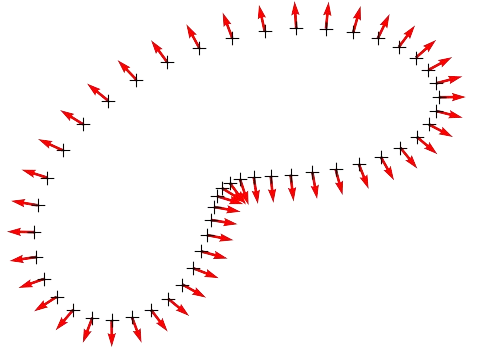
\includegraphics[width=7cm]{images/levelset/points_normals.png}};

\column{0.5}

\block{Numerical Results \textnormal{- Learn a complex levelset}}{
    \vspace{-20pt}
    \begin{center}
        \begin{tcolorbox}[
            colback=color1!50, % Couleur de fond de la boîte
            colframe=color2, % Couleur du cadre de la boîte
            arc=2mm, % Rayon de l'arrondi des coins
            boxrule=2pt, % Épaisseur du cadre de la boîte
            breakable, enhanced jigsaw,
            width=\linewidth
            ]            
            \textbf{Levelset learning.}

            \vspace{2pt}

            \begin{minipage}{0.48\linewidth}
                \centering
                \pgfimage[width=0.7\linewidth]{images/levelset/cat_levelset_loss.png}
            \end{minipage} 
            \begin{minipage}{0.48\linewidth}
                \centering
                \pgfimage[width=0.75\linewidth]{images/levelset/cat_levelset.png}
            \end{minipage} 
        \end{tcolorbox}

        \begin{tcolorbox}[
            colback=color1!50, % Couleur de fond de la boîte
            colframe=color2, % Couleur du cadre de la boîte
            arc=2mm, % Rayon de l'arrondi des coins
            boxrule=2pt, % Épaisseur du cadre de la boîte
            breakable, enhanced jigsaw,
            width=\linewidth
            ]            
            \textbf{Poisson problem on Cat.}

            \ding{217} Taking $f=1$ (\textbf{\fcolorbox{color1!50}{color1}{non parametric}}) and homogeneous Dirichlet BC ($g= 0$). \\
            \ding{217} Looking for $u_\theta = \phi w_\theta$ with $\phi$ the levelset learned.

            \vspace{2pt}

            \begin{minipage}{0.48\linewidth}
                \centering
                \pgfimage[width=0.7\linewidth]{images/levelset/cat_poisson_loss.png}
            \end{minipage} 
            \begin{minipage}{0.48\linewidth}
                \centering
                \pgfimage[width=0.9\linewidth]{images/levelset/cat_poisson.png}
            \end{minipage} 
        \end{tcolorbox}
    \end{center}
    \vspace{-30pt} 
}

\end{columns}

% \node (manote){
% };

% \begin{scope}[shift=(manote.south west), x={($0.1*(manote.south east)-0.1*(manote.south west)$)},
%      y={($0.1*(manote.north west)-0.1*(manote.south west)$)}]

%      \draw[lightgray, step=1](manote.south west) grid (manote.north east);

% \end{scope}

    
